% ============================================================
% Strict-Additive Fees Reinvested Inside Pricing for AMMs
% Two-Curve Design
% Author: Vadim Fadeev
% ============================================================
\documentclass[11pt]{article}

\usepackage[a4paper,margin=1in]{geometry}
\usepackage{amsmath,amssymb,amsthm,mathtools}
\usepackage{hyperref}
\usepackage{enumitem}
\usepackage{booktabs}
\usepackage{microtype}
\usepackage{tikz}
\usepackage{pgfplots}
\pgfplotsset{compat=1.17}

\hypersetup{colorlinks=true,linkcolor=blue,urlcolor=blue,citecolor=blue}

% theorem styles
\newtheorem{theorem}{Theorem}[section]
\newtheorem{lemma}[theorem]{Lemma}
\newtheorem{proposition}[theorem]{Proposition}
\newtheorem{corollary}[theorem]{Corollary}
\theoremstyle{definition}
\newtheorem{definition}[theorem]{Definition}
\theoremstyle{remark}
\newtheorem{remark}[theorem]{Remark}

% macros
\newcommand{\R}{\mathbb{R}}
\newcommand{\Rp}{\R_{>0}}
\newcommand{\dx}{\Delta x}
\newcommand{\dy}{\Delta y}
\newcommand{\projY}{\pi_y}

\title{\textbf{Strict-Additive Fees Reinvested Inside Pricing for AMMs}\\
\large Conservative and Dissipative Constructions with ExactIn/ExactOut}
\author{
  \begin{tabular}{@{}c@{\hspace{2em}}c@{}}
    Vadim Fadeev & Sergey Prilutskiy \\
    \texttt{xboxfadeev@gmail.com} & \texttt{prilutski@gmail.com} \\[1em]
    Vijay Singh & Sergej Kunz \\
    \texttt{vijaykumar.singh@openzeppelin.com} & \texttt{info@deacix.de}
  \end{tabular}
}
\date{\today}

\begin{document}
\maketitle

\paragraph{Acknowledgements.}
The authors thank
Nikita Galikhanov (n.galikhanov@1inch.io),
Gleb Alekseev (g.alekseev@1inch.io),
and Vasiliy Tikhonenko (v.tikhonenko@1inch.io)
for valuable discussions and feedback.

\begin{abstract}
Constant-product AMMs ($xy=k$) are strictly additive (split-invariant): executing a trade of size $a+b$ yields the same final pool state as executing $a$ and then $b$.
This paper studies fee mechanisms where fees are \emph{reinvested inside pricing} (no external fee buckets) while preserving strict additivity.
We show that strict additivity forces a telescoping structure that can be expressed as an invariant of the form $K=y\,\Psi(x)$.
This yields a \emph{conservative} design that is strictly additive for ExactIn and ExactOut and is invertible (a perfect round trip returns the pool to the start when the trader swaps back exactly what they received).
We then introduce a \emph{dissipative} design: a single deterministic mapping where the power $\alpha$ is always applied to the input token's reserve.
This mapping is strictly additive for splits in both directions, but is non-conservative---round trips cost the trader and accumulate value in reserves, creating a real bid-ask spread for economic incentive.
We prove an \emph{impossibility theorem}: no stateless fee mechanism can simultaneously be progressive (larger trades pay higher percentage) and LP-protective (splitting cannot reduce fees).
The dissipative design achieves statelessness and LP-protection at the cost of being anti-progressive; we quantify this trade-off with economic analysis and numerical evidence, and discuss alternative designs including cumulative volume fees.
We provide full intermediate derivations and numeric examples.
\end{abstract}

\tableofcontents

\section{Setup}

\begin{definition}[State]
The pool state is reserves $(x,y)\in\Rp^2$, where $x$ is token $X$ reserve and $y$ is token $Y$ reserve.
\end{definition}

\begin{definition}[State update map]
Let $F_\theta:\Rp^2\to\Rp^2$ be a state update map parameterized by a trade parameter $\theta$.
For ExactIn we take $\theta=\dx$; for ExactOut we take $\theta=\dy$.
We write
\[
F_\theta(x,y)=(x_\theta,y_\theta).
\]
\end{definition}

\begin{definition}[Strict additivity / split invariance]
A family $\{F_\theta\}$ is \emph{strictly additive} in parameter $\theta$ if for all $a,b>0$,
\[
F_{a+b} = F_b\circ F_a.
\]
Equivalently, applying $a$ then $b$ produces the same final state as applying $a+b$ once.
\end{definition}

\begin{definition}[Output function]
For ExactIn (parameter $\dx$), define
\[
\Delta y = f((x,y),\dx) := y-\projY(F_{\dx}(x,y)),
\]
where $\projY(x',y')=y'$.
\end{definition}

\section{Baseline: constant product $xy=k$}

\begin{lemma}[Constant product ExactIn]
With invariant $xy=k$ and full input credit $x'=x+\dx$, the post-swap $y$ is uniquely
\[
 y' = \frac{xy}{x+\dx} = y\frac{x}{x+\dx},
\]
and
\[
\Delta y_{\mathrm{cp}} = y-y' = y\frac{\dx}{x+\dx}.
\]
\end{lemma}

\begin{lemma}[Strict additivity for constant product]
Constant product is strictly additive for ExactIn.
\end{lemma}

\begin{proof}
Let $\dx=a+b$. After $a$, $y_1=xy/(x+a)$. After $b$, $y_2=(x+a)y_1/(x+a+b)=xy/(x+a+b)$, equal to the one-shot result.
\end{proof}

\section{Why the cocycle condition appears}

A common way to model reinvested fees is to start from constant product and multiply by a factor $R(x,\Delta)\ge 1$ that keeps extra $Y$ in the pool:
\[
 y'(x,\Delta) = y\frac{x}{x+\Delta}R(x,\Delta).
\]

\begin{theorem}[Strict additivity implies the cocycle identity]
The update rule
\[
F_\Delta(x,y)=\left(x+\Delta,\; y\frac{x}{x+\Delta}R(x,\Delta)\right)
\]
is strictly additive in $\Delta$ iff
\[
\boxed{R(x,a)R(x+a,b)=R(x,a+b)}\qquad\forall x,a,b>0.
\]
\end{theorem}

\begin{proof}
Split $\Delta=a+b$.
After $a$:
\[
 y_1 = y\frac{x}{x+a}R(x,a),\quad x_1=x+a.
\]
After $b$:
\[
 y_2 = y_1\frac{x_1}{x_1+b}R(x_1,b)
     = \Big(y\frac{x}{x+a}R(x,a)\Big)\frac{x+a}{x+a+b}R(x+a,b).
\]
Cancel $x+a$:
\[
 y_2 = y\frac{x}{x+a+b}R(x,a)R(x+a,b).
\]
One-shot:
\[
 y_S = y\frac{x}{x+a+b}R(x,a+b).
\]
Strict additivity requires $y_2=y_S$ for all $y>0$, hence the boxed identity.
\end{proof}

\section{From $R$ to $\Psi$: a better description of the potential function}

\subsection{Telescoping solution via an endpoint potential $G$}

\begin{theorem}[General telescoping form]
If the cocycle identity holds, then (under mild regularity) there exists $G:\Rp\to\Rp$ such that
\[
\boxed{R(x,\Delta)=\frac{G(x)}{G(x+\Delta)}}.
\]
Conversely, any such ratio satisfies the cocycle identity.
\end{theorem}

\begin{proof}
Sufficiency is immediate:
\[
\frac{G(x)}{G(x+a)}\cdot\frac{G(x+a)}{G(x+a+b)}=\frac{G(x)}{G(x+a+b)}.
\]
Necessity can be shown by fixing a reference point and defining $G$ by endpoint products so that intermediate factors cancel.
\end{proof}

\subsection{Defining $\Psi$ and its economic meaning}

Substitute $R(x,\Delta)=G(x)/G(x+\Delta)$:
\[
 y' = y\frac{x}{x+\Delta}\frac{G(x)}{G(x+\Delta)} = y\frac{xG(x)}{(x+\Delta)G(x+\Delta)}.
\]
Define the combined potential coordinate
\[
\boxed{\Psi(x):=xG(x)}.
\]
Then the update becomes
\begin{equation}
\boxed{\;x'=x+\Delta,\qquad y'=y\frac{\Psi(x)}{\Psi(x+\Delta)}.\;}
\label{eq:psi-exactin}
\end{equation}

\begin{proposition}[Invariant]
The quantity
\[
\boxed{K:=y\Psi(x)}
\]
is invariant under the update \eqref{eq:psi-exactin}.
\end{proposition}

\begin{proof}
Multiply both sides of \eqref{eq:psi-exactin} by $\Psi(x')=\Psi(x+\Delta)$:
\[
 y'\Psi(x') = y\frac{\Psi(x)}{\Psi(x')}\Psi(x') = y\Psi(x).
\]
\end{proof}

\begin{remark}[Economic interpretation of $\Psi$]
$\Psi$ is a monotone (typically increasing) re-parameterization of the $x$-reserve.
The swap outcome depends only on the endpoint ratio $\Psi(x)/\Psi(x')$.
You can interpret $\Psi(x)$ as the pool's \emph{effective} or \emph{virtual} $X$-liquidity coordinate.
A different $\Psi$ changes the curvature of the AMM and therefore changes how much output is paid for the same input.
\end{remark}

\begin{proposition}[Marginal price]
On the invariant curve $y\Psi(x)=K$, the instantaneous price (marginal $Y$ out per $X$ in) is
\[
\boxed{p(x,y)=-\frac{dy}{dx} = \frac{y\Psi'(x)}{\Psi(x)}.}
\]
\end{proposition}

\begin{proof}
Differentiate $y\Psi(x)=K$:
$\Psi(x)dy + y\Psi'(x)dx =0$. Rearranging yields the formula.
\end{proof}

\section{Conservative Design (Single Invariant)}

The conservative design uses one function $\Psi$ for both directions, i.e., one conserved quantity $K=y\Psi(x)$. It is strictly additive and invertible (time-reversible).

\subsection{ExactIn $X\to Y$}

From \eqref{eq:psi-exactin}, the output is
\begin{equation}
\boxed{\;\Delta y = y-y' = y\left(1-\frac{\Psi(x)}{\Psi(x+\dx)}\right).\;}
\label{eq:curveA-exactin-out}
\end{equation}

\subsection{ExactOut $X\to Y$: full derivation}

Given a target $0<\dy<y$, set $y'=y-\dy$.
Conservation of $K=y\Psi(x)$ implies
\[
 (y-\dy)\Psi(x') = y\Psi(x).
\]
Solve for $\Psi(x')$:
\[
 \Psi(x') = \Psi(x)\frac{y}{y-\dy}.
\]
Assuming $\Psi$ is invertible:
\[
 x' = \Psi^{-1}\!\left(\Psi(x)\frac{y}{y-\dy}\right),\qquad
 \boxed{\dx = x'-x = \Psi^{-1}\!\left(\Psi(x)\frac{y}{y-\dy}\right)-x.}
\]

\subsection{Strict additivity checks}

\begin{lemma}[ExactIn strict additivity for Curve A]
For all $a,b>0$,
\[
F^{A,\mathrm{in}}_{a+b} = F^{A,\mathrm{in}}_b\circ F^{A,\mathrm{in}}_a.
\]
\end{lemma}

\begin{proof}
After $a$: $y_1=y\Psi(x)/\Psi(x+a)$. After $b$: $y_2=y_1\Psi(x+a)/\Psi(x+a+b)=y\Psi(x)/\Psi(x+a+b)$.
\end{proof}

\begin{lemma}[ExactOut strict additivity for Curve A]
For $a,b>0$ with $a+b<y$, the ExactOut map is strictly additive in $\dy$.
\end{lemma}

\begin{proof}
Write $r(\dy)=y/(y-\dy)$. Note that $r(a)\,r(b\mid y-a)=y/(y-a)\cdot (y-a)/(y-a-b)=y/(y-a-b)=r(a+b)$.
Since ExactOut is $\Psi(x')=\Psi(x)r(\dy)$, endpoint multiplication yields the same $\Psi(x')$ and hence the same $x'$.
\end{proof}

\subsection{Why conservative design allows perfect round trips}

\begin{proposition}[Round trip is an identity (ideal real arithmetic)]
In the conservative design, perform ExactIn $X\to Y$ with input $\dx$ producing output $\dy$. Then input exactly that $\dy$ back in the reverse direction. The pool returns to the initial state (modulo rounding).
\end{proposition}

\begin{proof}
Both legs preserve the same invariant $K=y\Psi(x)$. After the first leg, the trader received $\dy=y-y'$. Inputting $\dy$ back restores $y$ to its initial value. With $y$ restored and $K$ unchanged, $\Psi(x)$ must also be restored, implying $x$ returns (for invertible $\Psi$).
\end{proof}

\subsection{Reinvested fee accounting relative to constant product}

For the same $\dx$, constant product yields $y_{\mathrm{cp}}=y\,x/(x+\dx)$. The conservative design yields $y'=y\Psi(x)/\Psi(x+\dx)$.
Define retained $Y$ vs constant product:
\[
\boxed{\mathrm{fee}_Y^{(\mathrm{vs\,CP})}=y' - y_{\mathrm{cp}} = y\left(\frac{\Psi(x)}{\Psi(x+\dx)}-\frac{x}{x+\dx}\right).}
\]
This quantity measures how much more $Y$ remains in the pool compared to pure constant product for the same input.

\section{Conservative power family: $\Psi(x)=x^\alpha$}

Let $0<\alpha\le 1$ and $\Psi(x)=x^\alpha$. Then invariant is
\[
\boxed{K=x^\alpha y.}
\]
ExactIn output is
\[
\boxed{\Delta y = y\left(1-\left(\frac{x}{x+\dx}\right)^\alpha\right).}
\]
ExactOut input for target $\dy$ is
\[
\boxed{\dx = x\left(\left(\frac{y}{y-\dy}\right)^{1/\alpha}-1\right).}
\]
Marginal price becomes
\[
\boxed{p=\alpha\frac{y}{x}.}
\]


\paragraph{Implementation formulas (ExactIn / ExactOut).}
For on-chain implementations it is useful to expose closed forms for both swap directions.
We write the trader input as \(\dx_{\mathrm{in}}\) or \(\dy_{\mathrm{in}}\) and the trader output as \(\dy_{\mathrm{out}}\) or \(\dx_{\mathrm{out}}\).

\textbf{(i) \(X \to Y\) direction.}
\begin{align}
\textbf{ExactIn:}\quad
\dy_{\mathrm{out}}
&= y - y'
= y\left(1 - \left(\frac{x}{x+\dx_{\mathrm{in}}}\right)^{\alpha}\right),
\\[4pt]
\textbf{ExactOut:}\quad
\dx_{\mathrm{in}}
&= x\left(\left(\frac{y}{y-\dy_{\mathrm{out}}}\right)^{1/\alpha}-1\right),
\qquad 0<\dy_{\mathrm{out}}<y.
\end{align}

\textbf{(ii) \(Y \to X\) direction.}
\begin{align}
\textbf{ExactIn:}\quad
\dx_{\mathrm{out}}
&= x - x'
= x\left(1 - \left(\frac{y}{y+\dy_{\mathrm{in}}}\right)^{\alpha}\right),
\\[4pt]
\textbf{ExactOut:}\quad
\dy_{\mathrm{in}}
&= y\left(\left(\frac{x}{x-\dx_{\mathrm{out}}}\right)^{1/\alpha}-1\right),
\qquad 0<\dx_{\mathrm{out}}<x.
\end{align}

\section{Dissipative Design (Single Deterministic Mapping)}

The dissipative design uses a \emph{single} mapping rule: the power $\alpha$ is always applied to the \textbf{input token's reserve}.
This is not two separate curves, but one unified, asymmetric mapping that is non-conservative (dissipative).

\subsection{The unified dissipative mapping}

The key insight is that there is \textbf{one rule}: when token $T$ is input, apply $\Psi_T(t)=t^\alpha$ to its reserve.
This yields a single parameterized family of state updates:
\[
\boxed{F_{\Delta_{\mathrm{in}}}(x,y)=\begin{cases}
\left(x+\dx,\;y\left(\dfrac{x}{x+\dx}\right)^\alpha\right) & \text{when $X$ is input,}\\[1em]
\left(x\left(\dfrac{y}{y+\dy}\right)^\alpha,\;y+\dy\right) & \text{when $Y$ is input.}
\end{cases}}
\]
Each direction is strictly additive in its own input parameter by telescoping.

\subsection{Why ``dissipative'' is the right framing}

\begin{itemize}
\item \textbf{Single rule}: Power the input token's reserve ratio---one formula, not two curves.
\item \textbf{Deterministic}: Given (state, input, direction), output is uniquely determined.
\item \textbf{Non-conservative}: Round trips lose value (like friction in physics).
\item \textbf{Time-irreversible}: Unlike conservative Hamiltonian systems, you cannot reverse time to recover the initial state.
\end{itemize}

\subsection{Symmetric power example: $\Psi(t)=t^\alpha$}

With $0<\alpha<1$:
\[
X\to Y:\quad y' = y\left(\frac{x}{x+\dx}\right)^\alpha.
\]
\[
Y\to X:\quad x' = x\left(\frac{y}{y+\dy}\right)^\alpha.
\]
Unlike the conservative design, these directions do not preserve a single global $K$, so round trips dissipate trader value into the pool.


\paragraph{Implementation formulas (ExactIn / ExactOut).}
Even though this section defines a \emph{dissipative} mapping (no invariant), the per-swap
closed forms are identical to Section~6, because each direction still follows the same one-step
update rule.

\textbf{(i) \(X \to Y\) direction.}
\begin{align}
\textbf{ExactIn:}\quad
\dy_{\mathrm{out}}
&= y - y'
= y\left(1 - \left(\frac{x}{x+\dx_{\mathrm{in}}}\right)^{\alpha}\right),
\\[4pt]
\textbf{ExactOut:}\quad
\dx_{\mathrm{in}}
&= x\left(\left(\frac{y}{y-\dy_{\mathrm{out}}}\right)^{1/\alpha}-1\right),
\qquad 0<\dy_{\mathrm{out}}<y.
\end{align}

\textbf{(ii) \(Y \to X\) direction.}
\begin{align}
\textbf{ExactIn:}\quad
\dx_{\mathrm{out}}
&= x - x'
= x\left(1 - \left(\frac{y}{y+\dy_{\mathrm{in}}}\right)^{\alpha}\right),
\\[4pt]
\textbf{ExactOut:}\quad
\dy_{\mathrm{in}}
&= y\left(\left(\frac{x}{x-\dx_{\mathrm{out}}}\right)^{1/\alpha}-1\right),
\qquad 0<\dx_{\mathrm{out}}<x.
\end{align}

\section{Why Strict Additivity Matters}\label{sec:why-sa}

A natural question is why strict additivity (split-invariance) should be a design goal at all.
After all, the standard Curve-style output-fee rule is \emph{superadditive}: splitting a trade yields strictly \emph{more} output than one-shot execution, which is ``good for traders.''
However, superadditivity still creates path dependence, which has concrete negative consequences.

\subsection{Formal additivity types for trader output}

\begin{definition}[Additivity types]\label{def:additivity-types}
Let $\mathrm{Out}(\Delta;x,y):= y - \projY(F_\Delta(x,y))$ be the trader output and
\[
\mathrm{Out}_{\mathrm{split}}(a,b;x,y) := \mathrm{Out}(a;x,y) + \mathrm{Out}(b;\,F_a(x,y))
\]
the total output from executing $a$ then $b$. The mechanism is:
\begin{enumerate}[label=(\alph*)]
\item \textbf{Strictly additive} if $\mathrm{Out}(a{+}b) = \mathrm{Out}_{\mathrm{split}}(a,b)$ for all $a,b\ge 0$. (Path-independent.)
\item \textbf{Subadditive} if $\mathrm{Out}(a{+}b) > \mathrm{Out}_{\mathrm{split}}(a,b)$ for all $a,b>0$. (One-shot is better; splitting hurts the trader.)
\item \textbf{Superadditive} if $\mathrm{Out}(a{+}b) < \mathrm{Out}_{\mathrm{split}}(a,b)$ for all $a,b>0$. (Split is better; one-shot hurts the trader.)
\end{enumerate}
\end{definition}

\subsection{How standard fee rules break strict additivity on $xy=k$}

Both common fee mechanisms applied to constant product create path dependence:

\paragraph{Output-fee (Curve-style) is superadditive.}
Start from $(x,y)$ with $k=xy$. The fee-free output for input $\Delta$ is $\Delta y_{\mathrm{nf}} = y\Delta/(x{+}\Delta)$.
The rule: pay trader $(1{-}f)\Delta y_{\mathrm{nf}}$ and keep $f\Delta y_{\mathrm{nf}}$ in $Y$.
After the trade, $y_1 = xy/(x{+}\Delta) + fy\Delta/(x{+}\Delta)= y(x{+}f\Delta)/(x{+}\Delta)$, so
\[
k_1 = (x{+}\Delta)\,y_1 = y(x + f\Delta) > xy = k_0.
\]
The fee pushes $k$ upward. The second chunk of a split trade executes on a ``richer'' pool (higher $k$), yielding more output than the corresponding portion of a one-shot trade.
Splitting is strictly better for the trader: \emph{superadditive}.

\paragraph{Input-fee reinvest is subadditive.}
Trade only the net amount $(1{-}f)\Delta$ on the constant-$k$ curve: $y_{\mathrm{nf}} = xy/(x{+}(1{-}f)\Delta)$.
Credit the full $\Delta$ to reserves: $x_1 = x+\Delta$.
Now $k_1 = x_1\,y_{\mathrm{nf}} = (x{+}\Delta)\cdot xy/(x{+}(1{-}f)\Delta) > xy$ since $x{+}\Delta > x{+}(1{-}f)\Delta$.
The extra $X$ makes the pool more $X$-heavy; subsequent $X\to Y$ trades face worse terms.
Splitting is strictly worse for the trader: \emph{subadditive}.

\paragraph{Dissipative $r^\alpha$ is strictly additive.}
By telescoping (Section~4), the outcome depends only on the ratio $\Psi(x)/\Psi(x{+}\Delta)$.
Intermediate terms cancel identically regardless of how $\Delta$ is split.
There is no path dependence: \emph{strictly additive}.

\subsection{Why path-independence is the right design goal}

\begin{enumerate}[label=(\alph*)]
\item \textbf{Aggregator/router neutrality.}
If the swap outcome depends on how execution is split, routing algorithms must simulate all possible split patterns to find the optimal one.
Strict additivity means routers can split arbitrarily without affecting the final outcome---the optimization problem collapses.

\item \textbf{Partial fills and TWAP.}
Time-weighted execution, partial limit-order fills, and MEV-resistant chunking all require that outcome does not depend on chunking granularity.
With superadditive fees, a TWAP order gets a different outcome depending on chunk sizes---an undesirable property.

\item \textbf{Deterministic pool growth.}
Under strict additivity, the pool's effective liquidity grows deterministically with volume, independent of how trades are split.
This makes LP returns predictable from aggregate volume alone.

\item \textbf{Composability.}
Protocols building on top of the AMM (vaults, strategies, aggregators) can reason about outcomes without simulating all possible split patterns.

\item \textbf{No gaming incentive.}
With superadditive fees, sophisticated traders split trades to gain advantage. With subadditive fees, they batch.
Both create unfair advantages. Strict additivity eliminates the gaming dimension entirely.
\end{enumerate}

\begin{remark}[SwapVM compatibility]
In the SwapVM architecture, orders are bytecode programs executed by an on-chain VM.
Each program specifies its pricing instruction (e.g., dissipative power-curve swap).
Strict additivity ensures that the program's economic outcome is independent of how the taker chooses to fill the order---critical for a system where makers publish programs and takers execute them.
\end{remark}

\begin{center}
\begin{tabular}{@{}lllll@{}}
\toprule
\textbf{Fee Rule} & \textbf{Additivity} & \textbf{For Trader} & \textbf{Path-Dep.?} & \textbf{$k$ Change} \\
\midrule
Fee-free $xy=k$ & Strictly additive & Path-independent & No & $k$ constant \\
Output-fee (Curve) & Superadditive & Split better & Yes & $k$ increases (in $Y$) \\
Input-fee reinvest & Subadditive & One-shot better & Yes & $k$ increases (in $X$) \\
Dissipative $r^\alpha$ & Strictly additive & Path-independent & No & $K=y x^\alpha$ constant \\
\bottomrule
\end{tabular}
\end{center}


\section{The Impossibility Theorem}\label{sec:impossibility}

We now prove that the dissipative design's anti-progressive fee structure is not a design flaw but a \emph{mathematical necessity}: no stateless fee mechanism can simultaneously be progressive and LP-protective.

\subsection{Formal definitions}

\begin{definition}[Fee function]
A \emph{fee function} is a mapping $f:\Rp\times\mathcal{S}\to\R_{\ge 0}$ where $\Delta\in\Rp$ is the trade size, $s\in\mathcal{S}$ is the system state, and $f(\Delta,s)$ is the fee charged.
\end{definition}

\begin{definition}[Stateless]
A fee function is \emph{stateless} if $s$ consists only of the current reserves $(x,y)$:
$f(\Delta,s)=f(\Delta,x,y)$.
No historical information is required.
\end{definition}

\begin{definition}[Progressive]
A fee function is \emph{progressive} if the fee rate $\varphi(\Delta,s):=f(\Delta,s)/\Delta$ is strictly increasing in $\Delta$ at fixed $s$:
\[
\Delta_2 > \Delta_1 \;\Longrightarrow\; \frac{f(\Delta_2,s)}{\Delta_2} > \frac{f(\Delta_1,s)}{\Delta_1}.
\]
\end{definition}

\begin{definition}[LP-Protective]
A fee function is \emph{LP-protective} if splitting a trade cannot reduce the total fee:
\[
f(a+b,\,s) \;\le\; f(a,\,s) + f(b,\,s_a)
\]
where $s_a$ is the state after executing trade $a$.
\end{definition}

\subsection{Key lemma: progressive implies superadditivity at fixed state}

\begin{lemma}\label{lem:prog-super}
If a fee function $f$ is progressive, then at any fixed state $s$:
\[
f(a+b,\,s) > f(a,\,s) + f(b,\,s) \qquad\forall\, a,b>0.
\]
\end{lemma}

\begin{proof}
Let $\varphi(\Delta):=f(\Delta,s)/\Delta$. Progressive means $\varphi$ is strictly increasing, so $\varphi(a+b)>\varphi(a)$ and $\varphi(a+b)>\varphi(b)$. Then:
\[
f(a+b) = a\,\varphi(a+b) + b\,\varphi(a+b) > a\,\varphi(a) + b\,\varphi(b) = f(a)+f(b). \qedhere
\]
\end{proof}

\subsection{Main theorem}

\begin{theorem}[Impossibility of Stateless $+$ Progressive $+$ LP-Protective]\label{thm:impossibility}
There exists no fee function that is simultaneously stateless, progressive, and LP-protective.
\end{theorem}

\begin{proof}
Suppose for contradiction that such a function $f$ exists.
Fix a state $s_0$ and a total trade size $D>0$.
Split $D$ into $n$ equal pieces of size $D/n$ and let $s_i$ denote the state after the $i$-th sub-trade.

\medskip\noindent
\textbf{Step 1 (LP-protective gives an upper bound).}
Applying the LP-protective inequality $n-1$ times:
\begin{equation}\label{eq:lp-split}
f(D,\,s_0) \;\le\; \sum_{i=0}^{n-1} f\!\left(\frac{D}{n},\,s_i\right).
\end{equation}

\medskip\noindent
\textbf{Step 2 (State changes are second-order for small sub-trades).}
Since $f$ is stateless, $s_i$ depends only on current reserves.
After $i$ sub-trades of size $D/n$, the reserves have shifted by a total of $iD/n$.
For a smooth fee function, Taylor expansion gives:
\[
f\!\left(\frac{D}{n},\,s_i\right) = f\!\left(\frac{D}{n},\,s_0\right) + O\!\left(\frac{D^2}{n^2}\right).
\]

Summing over $n$ terms:
\[
\sum_{i=0}^{n-1} f\!\left(\frac{D}{n},\,s_i\right) = n\cdot f\!\left(\frac{D}{n},\,s_0\right) + O\!\left(\frac{D^2}{n}\right)
= D\cdot\varphi\!\left(\frac{D}{n},\,s_0\right) + O\!\left(\frac{D^2}{n}\right).
\]

\medskip\noindent
\textbf{Step 3 (Progressive rate reduction is first-order).}
Since $\varphi$ is strictly increasing in $\Delta$ and $D/n < D$ for $n\ge 2$:
\[
\varphi\!\left(\frac{D}{n},s_0\right) < \varphi(D,s_0).
\]
Taking $n\to\infty$:
\[
\lim_{n\to\infty}\left[D\cdot\varphi\!\left(\frac{D}{n},s_0\right) + O\!\left(\frac{D^2}{n}\right)\right]
= D\cdot\varphi(0^+,s_0) < D\cdot\varphi(D,s_0) = f(D,s_0).
\]

\medskip\noindent
\textbf{Step 4 (Contradiction).}
For sufficiently large $n$, the right side of \eqref{eq:lp-split} is strictly less than $f(D,s_0)$, contradicting \eqref{eq:lp-split}.
\end{proof}

\begin{remark}[Why this proof handles state changes correctly]
Unlike the na\"ive argument that reduces LP-protection to same-state subadditivity $f(a+b)\le f(a)+f(b)$ (which is valid only when state doesn't change between sub-trades), this proof accounts for state evolution.
The key insight is that for infinitesimal splits, state changes are \emph{second-order} ($O(D^2/n^2)$ per step, $O(D^2/n)$ total), while the progressive rate reduction from $\varphi(D)$ to $\varphi(D/n)$ is \emph{first-order}.
\end{remark}

\begin{corollary}[Design space constraint]\label{cor:design-space}
Any practical stateless fee mechanism must sacrifice either progressivity or LP-protection:
\begin{center}
\begin{tabular}{@{}lcccl@{}}
\toprule
\textbf{Design} & \textbf{Stateless} & \textbf{Progressive} & \textbf{LP-Protective} & \textbf{Sacrifice} \\
\midrule
Flat fee & \checkmark & --- & \checkmark & Progressive \\
Dissipative $r^\alpha$ & \checkmark & $\times$ (anti) & \checkmark & Progressive \\
Per-trade progressive & \checkmark & \checkmark & $\times$ & LP-Protective \\
Cumulative volume & $\times$ & \checkmark & \checkmark & Stateless \\
\bottomrule
\end{tabular}
\end{center}
The dissipative design occupies the ``stateless $+$ LP-protective'' cell, necessarily sacrificing progressivity.
\end{corollary}

\subsection{Geometric interpretation}

\begin{figure}[htbp]
\centering
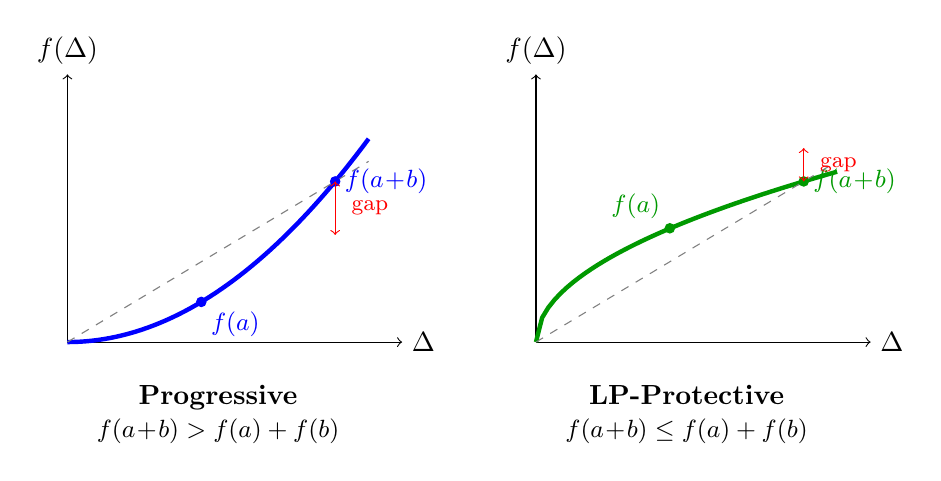
\begin{tikzpicture}[scale=0.85]
    \begin{scope}[xshift=0cm]
        \draw[->] (0,0) -- (5,0) node[right] {$\Delta$};
        \draw[->] (0,0) -- (0,4) node[above] {$f(\Delta)$};
        \draw[blue, ultra thick, domain=0:4.5, samples=50] plot (\x, {0.15*\x*\x});
        \draw[gray, dashed] (0,0) -- (4.5, 2.7);
        \filldraw[blue] (2, 0.6) circle (2pt) node[below right] {\small$f(a)$};
        \filldraw[blue] (4, 2.4) circle (2pt) node[right] {\small$f(a\!+\!b)$};
        \draw[<->, red] (4, 1.6) -- (4, 2.4);
        \node[red, right] at (4.1, 2.0) {\footnotesize gap};
        \node[below] at (2.25, -0.5) {\textbf{Progressive}};
        \node[below] at (2.25, -1) {\small $f(a\!+\!b) > f(a)+f(b)$};
    \end{scope}
    \begin{scope}[xshift=7cm]
        \draw[->] (0,0) -- (5,0) node[right] {$\Delta$};
        \draw[->] (0,0) -- (0,4) node[above] {$f(\Delta)$};
        \draw[green!60!black, ultra thick, domain=0:4.5, samples=50] plot (\x, {1.2*sqrt(\x)});
        \draw[gray, dashed] (0,0) -- (4.5, 2.7);
        \filldraw[green!60!black] (2, 1.7) circle (2pt) node[above left] {\small$f(a)$};
        \filldraw[green!60!black] (4, 2.4) circle (2pt) node[right] {\small$f(a\!+\!b)$};
        \draw[<->, red] (4, 2.4) -- (4, 2.9);
        \node[red, right] at (4.1, 2.65) {\footnotesize gap};
        \node[below] at (2.25, -0.5) {\textbf{LP-Protective}};
        \node[below] at (2.25, -1) {\small $f(a\!+\!b) \le f(a)+f(b)$};
    \end{scope}
\end{tikzpicture}
\caption{Progressive fees are convex (superadditive at fixed state), while LP-protective fees are concave (subadditive). No function can be both.}
\label{fig:impossibility-geometry}
\end{figure}

\subsection{Information-theoretic intuition}

The impossibility has a clean information-theoretic interpretation:
\begin{enumerate}
\item \textbf{Progressive} requires ``knowing'' a trade is large $\rightarrow$ charge more.
\item \textbf{LP-Protective} means the mechanism cannot distinguish a single large trade from many small trades (split-invariant).
\item \textbf{Stateless} means no memory of previous trades.
\end{enumerate}
If the mechanism cannot distinguish large from split-small (LP-protective) and has no memory (stateless), it \emph{cannot know} a trade is large (progressive).
Changing the AMM curve does not create information that doesn't exist---the constraint is fundamental, not formula-specific.

\subsection{Can changing the curve escape the impossibility?}

As proven in Sections~3--4, \emph{any} monotone $\Psi:\Rp\to\Rp$ yields a strictly additive (telescoping) invariant $K=y\Psi(x)$.
Telescoping gives LP-protection for free.
The question is whether some non-power $\Psi$ can achieve progressive implicit fees.

\begin{theorem}[Anti-progressive structure for general $\Psi$]\label{thm:impossibility-general-psi}
For any potential function $\Psi$ with positive implicit fees (i.e., the trader receives less than constant product), the fee structure is anti-progressive.
\end{theorem}

\begin{proof}
The curve gives output $\dy = y(1-\Psi(x)/\Psi(x+\Delta))$.
When a trade of size $\Delta$ executes, the $x$-reserve moves from $x$ to $x+\Delta$.
The \emph{marginal implicit fee rate} at reserve level $x$ is the infinitesimal fee per unit input:
\[
\mu(x) := \lim_{\delta\to 0}\frac{\text{fee}(\delta;\,x)}{y\,\delta}
= \frac{1}{x} - \frac{\Psi'(x)}{\Psi(x)}.
\]
(This follows from L'H\^{o}pital on the difference between constant-product and $\Psi$-curve outputs.)
Positive fees require $\mu(x)>0$, i.e., $\Psi'(x)/\Psi(x) < 1/x$, meaning $\Psi$ grows slower than linear.

For the overall fee to be \emph{progressive} in trade size, $\mu(x)$ must be increasing in $x$ (so that later units of a large trade pay more than earlier units).
Differentiating:
\[
\mu'(x) = -\frac{1}{x^2} - \frac{\Psi''\Psi - (\Psi')^2}{\Psi^2}.
\]
Substituting $\Psi=e^g$ (so $\Psi'/\Psi=g'$ and $(\Psi''\Psi-(\Psi')^2)/\Psi^2 = g''$):
\[
\mu'(x) = -\frac{1}{x^2} - g''.
\]
Progressive requires $\mu'>0$, i.e., $g'' < -1/x^2$.

At the boundary $g''=-1/x^2$, integrating gives $g=\ln x + cx + c_0$, so $\Psi(x)=Axe^{cx}$.
For this boundary function, $\mu(x) = 1/x - (1/x + c) = -c$.
Positive fees require $\mu>0$, hence $c<0$.

Moving past the boundary to the progressive side ($g'' < -1/x^2$) requires $c>0$, but $c>0$ gives $\mu = -c < 0$---negative fees.
The boundary between progressive and anti-progressive coincides exactly with zero fees: no $\Psi$ can have both positive fees and progressive structure.
\end{proof}

\begin{theorem}[Ratio-only dependence requires power functions]\label{thm:ratio-only}
For $\Psi(x)/\Psi(x+\Delta)$ to depend only on the reserve ratio $r=x/(x+\Delta)$ (and not on $x$ independently), we must have $\Psi(x)=Ax^\alpha$.
\end{theorem}

\begin{proof}
Require $\Psi(x)/\Psi(x+\Delta)=g(r)$ for some function $g$.
Since $x+\Delta=x/r$, substituting $u=x/r$ gives $\Psi(ur)/\Psi(u)=g(r)$.
Taking $h=\ln\Psi$: $h(ur)-h(u)=\ln g(r)$.
Setting $u=1$: $h(r)-h(1)=\ln g(r)$.
With $H(x):=h(x)-h(1)$, this becomes $H(ur)=H(u)+H(r)$---Cauchy's multiplicative equation.
The continuous solutions are $H(x)=\alpha\ln x$, giving $\Psi(x)=Ax^\alpha$.
\end{proof}

\begin{remark}
Ratio-only dependence ensures \emph{scale invariance}: a 10\% trade has the same fee rate regardless of pool size.
This is the property that singles out power functions---not telescoping, which holds for any $\Psi$.
\end{remark}


\section{Economic Analysis of the Dissipative Design}\label{sec:economic}

We now quantify the anti-progressive structure implied by the impossibility theorem for the dissipative power-curve design.

\subsection{Effective fee rate}

\begin{definition}[Effective fee rate vs constant product]
For a dissipative swap with reserve ratio $r=x/(x+\dx)\in(0,1)$ and power $\alpha\in(0,1)$, the fraction of constant-product output retained by the pool is:
\begin{equation}\label{eq:phi-eff}
\varphi_{\mathrm{eff}}(r) = \frac{r^\alpha - r}{1-r}.
\end{equation}
\end{definition}

\begin{theorem}[Anti-progressive structure]\label{thm:anti-prog}
For $0<\alpha<1$, $\varphi_{\mathrm{eff}}$ is strictly decreasing in trade size (i.e., increasing in $r$):
\begin{itemize}
\item As $r\to 1$ (small trades): $\varphi_{\mathrm{eff}}\to 1-\alpha$.
\item As $r\to 0$ (large trades): $\varphi_{\mathrm{eff}}\to 0$.
\end{itemize}
\end{theorem}

\begin{proof}
The small-trade limit follows by L'H\^{o}pital's rule:
$\lim_{r\to 1}(r^\alpha-r)/(1-r) = \lim_{r\to 1}(\alpha r^{\alpha-1}-1)/(-1)=1-\alpha$.
The large-trade limit is immediate: $(0-0)/1=0$.
For the intermediate range, expand $r^\alpha = r\cdot e^{(\alpha-1)\ln r} \approx r(1+(\alpha-1)\ln r)$ for $\alpha$ near 1, giving $\varphi_{\mathrm{eff}}\approx (1-\alpha)\cdot r|\ln r|/(1-r)$, which decreases as $r$ decreases (trade size increases) because the $r$ factor dominates $|\ln r|$.
\end{proof}

\subsection{Fee rate by trade size ($\alpha=0.997$)}

For $\alpha=0.997$ (targeting $\sim\!0.3\%$ fee on small trades) with pool reserves $x=y=1000$:

\begin{center}
\begin{tabular}{@{}cccccc@{}}
\toprule
\textbf{Trade Size} & $\dx$ & $r$ & $\dy_{\mathrm{cp}}$ & \textbf{Fee Rate} & \textbf{vs 1\%} \\
\midrule
1\% of pool & 10 & 0.9901 & 9.901 & 0.299\% & --- \\
5\% of pool & 50 & 0.9524 & 47.619 & 0.293\% & $-2.0\%$ \\
10\% of pool & 100 & 0.9091 & 90.909 & 0.286\% & $-4.3\%$ \\
20\% of pool & 200 & 0.8333 & 166.667 & 0.271\% & $-9.4\%$ \\
50\% of pool & 500 & 0.6667 & 333.333 & 0.243\% & $-18.7\%$ \\
\bottomrule
\end{tabular}
\end{center}

The ``vs 1\%'' column shows the percentage reduction in fee rate compared to the smallest trade.
Typical arbitrage trades (10--20\% of pool) receive a $\sim\!5\text{--}10\%$ fee discount; this is modest but systematic.

\subsection{Comparison with alternative fee mechanisms}

\begin{center}
\begin{tabular}{@{}lcccc@{}}
\toprule
\textbf{Trade Size} & \textbf{Flat Fee} & \textbf{Dissipative} & \textbf{Progressive}$^*$ & \textbf{Desired Direction} \\
\midrule
1\% & 0.30\% & 0.30\% & 0.30\% & Low \\
10\% & 0.30\% & 0.29\% & 0.35\% & Medium \\
20\% & 0.30\% & 0.27\% & 0.45\% & Higher \\
50\% & 0.30\% & 0.24\% & 0.80\% & High \\
\bottomrule
\end{tabular}
\end{center}
\textit{$^*$Progressive fees are illustrative (e.g., cumulative volume approach).}

\subsection{Alternative: cumulative volume design}

The impossibility theorem (Theorem~\ref{thm:impossibility}) shows that achieving progressive $+$ LP-protective requires state.
The simplest such design tracks \emph{cumulative volume} $V$ per pool:
\[
f(\Delta;\,V) = F(V+\Delta) - F(V),
\]
where $F$ is convex (e.g., $F(V)=\kappa V^2$).
The marginal fee rate $F'(V)$ increases with $V$, giving progressivity.
Telescoping gives LP-protection: splits sum to the same total by construction.

\textbf{Cost:} One storage slot per pool (or per order, in the SwapVM setting).

\textbf{Benefit:} Progressive $+$ LP-protective.

\subsection{Why stateless is preferred for the dissipative design}

Despite the alternative, we adopt the stateless dissipative design for the following reasons:

\begin{enumerate}
\item \textbf{Gas cost.}
Each storage write (SSTORE) costs $\sim\!20{,}000$ gas on initial write, $\sim\!5{,}000$ on update.
The dissipative design requires \emph{zero} additional storage---the output is computed purely from reserves and $\alpha$.

\item \textbf{SwapVM compatibility.}
In the SwapVM architecture, pricing instructions execute within a bytecode VM.
Adding per-order or per-pool storage for cumulative volume would require new opcodes, storage management, and garbage collection logic.
The stateless design fits naturally as a pure-function instruction.

\item \textbf{Simplicity and auditability.}
The entire fee mechanism is a single formula: $y'=y(x/(x+\dx))^\alpha$.
There is no state to initialize, decay, or migrate.

\item \textbf{Modest practical impact.}
Within the realistic trade range (1--20\% of pool), the anti-progressive discount is $\le 10\%$.
For most maker strategies, this is an acceptable trade-off against the benefits above.
\end{enumerate}

\begin{remark}[When to prefer cumulative volume]
If a pool consistently faces large arbitrage trades ($>20\%$ of reserves) and LP protection is the top priority, the cumulative volume approach may be preferable despite the storage cost.
The choice is a design parameter, not a correctness issue.
\end{remark}


\section{Numeric showcase and evidence}
We provide concrete numeric examples (with fully expanded calculations), a fee-rate visualization, and a round-trip loss summary.

\subsection{Fee rate vs trade size ($\alpha=0.997$)}

\begin{figure}[htbp]
\centering
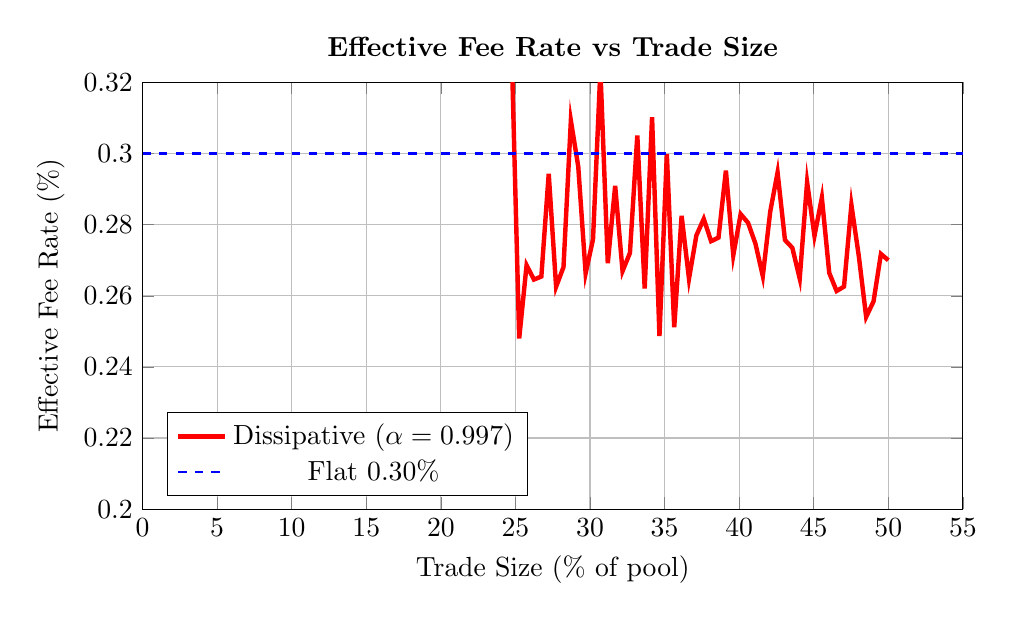
\begin{tikzpicture}
\begin{axis}[
    title={\textbf{Effective Fee Rate vs Trade Size}},
    xlabel={Trade Size (\% of pool)},
    ylabel={Effective Fee Rate (\%)},
    xmin=0, xmax=55,
    ymin=0.20, ymax=0.32,
    legend pos=south west,
    grid=major,
    width=12cm, height=7cm
]
\addplot[color=red, ultra thick, domain=1:50, samples=100]
    {100 * ((100/(100+x))^0.997 - (100/(100+x))) / (1 - (100/(100+x)))};
\addlegendentry{Dissipative ($\alpha=0.997$)}

\addplot[color=blue, thick, dashed, domain=0:55] {0.3};
\addlegendentry{Flat 0.30\%}
\end{axis}
\end{tikzpicture}
\caption{The effective fee rate decreases as trade size increases (anti-progressive). For $\alpha=0.997$, the fee drops from $\sim\!0.30\%$ for small trades to $\sim\!0.24\%$ at 50\% of pool. The dashed line shows a flat 0.30\% fee for comparison.}
\label{fig:fee-rate}
\end{figure}

\subsection{Round-trip loss summary ($\alpha=0.997$)}

The dissipative design collects fees through round-trip dissipation: a trader who buys $Y$ and immediately sells it back receives less $X$ than they started with.

\begin{center}
\begin{tabular}{@{}cccc@{}}
\toprule
\textbf{Trade Size} & \textbf{Trader Receives Back} & \textbf{Round-Trip Loss} & \textbf{Annualized Fee} \\
\midrule
$\dx=10$ (1\%) & $\approx 9.994$ & $\approx 0.06\%$ & $\sim\!0.6\%$ \\
$\dx=100$ (10\%) & $\approx 99.43$ & $\approx 0.57\%$ & $\sim\!0.57\%$ \\
$\dx=200$ (20\%) & $\approx 198.9$ & $\approx 0.55\%$ & $\sim\!0.55\%$ \\
\bottomrule
\end{tabular}
\end{center}

The round-trip loss is approximately $2(1-\alpha)\approx 0.6\%$ for small trades (twice the one-way fee), decreasing slightly for larger trades due to the anti-progressive structure.

\subsection{Detailed hand-checkable examples}

\paragraph{Example 1 (not strict additive):} Let \(x=y=1000\), \(\alpha=0.8\), and swap \(\dx_{\mathrm{in}}=100\) in the \(X\to Y\) direction.
\begin{align*}
\text{(CP baseline)}\quad
y' &= \frac{xy}{x+\dx_{\mathrm{in}}} = \frac{1000\cdot 1000}{1100} = \frac{1{,}000{,}000}{1100} \approx 909.0909090909,\\
\dy_{\mathrm{out}}^{\mathrm{CP}} &= 1000 - y' \approx 90.9090909091.
\end{align*}
For the power rule (Sections~6--7):
\begin{align*}
r &= \frac{x}{x+\dx_{\mathrm{in}}} = \frac{1000}{1100}=\frac{10}{11}\approx 0.9090909090909,\\
\ln r &\approx -0.0953101798043,\\
r^{0.8} &= \exp(0.8\ln r)=\exp\!\big(-0.0762481438435\big)\approx 0.9265862513559,\\
y_1 &= 1000\,r^{0.8} \approx 926.5862513558695,\\
\dy_{\mathrm{out}} &= 1000 - y_1 \approx 73.4137486441305.
\end{align*}
If we now swap back \(Y\to X\) by inputting \(\dy_{\mathrm{in}}=\dy_{\mathrm{out}}\) so that \(y_2=1000\), the update gives
\begin{align*}
\left(\frac{y_1}{1000}\right)^{0.8}
&= \exp\!\Big(0.8\ln\!\big(\tfrac{y_1}{1000}\big)\Big)
= \exp\!\big(-0.0609985150748\big)\approx 0.9408246368292,\\
x_2 &= 1100\left(\frac{y_1}{1000}\right)^{0.8} \approx 1034.9071005121361,\\
\dx_{\mathrm{back}} &= 1100-x_2 \approx 65.0928994878639.
\end{align*}
Here \(\dx_{\mathrm{back}}<100\), so doing the round trip loses value (not strict additive).

\paragraph{Example 2 (close to strict additive):} Same setup, but \(\alpha=0.997\).
\begin{align*}
r^{0.997} &= \exp(0.997\ln r)=\exp\!\big(-0.0950242492649\big)\approx 0.9093508831104,\\
y_1 &= 1000\,r^{0.997} \approx 909.3508831104054,\\
\dy_{\mathrm{out}} &= 1000-y_1 \approx 90.6491168895946.
\end{align*}
Swap back \(Y\to X\) with \(\dy_{\mathrm{in}}=\dy_{\mathrm{out}}\):
\begin{align*}
\left(\frac{y_1}{1000}\right)^{0.997}
&= \exp\!\Big(0.997\ln\!\big(\tfrac{y_1}{1000}\big)\Big)
= \exp\!\big(-0.0947391765171\big)\approx 0.9096101512187,\\
x_2 &= 1100\left(\frac{y_1}{1000}\right)^{0.997} \approx 1000.5711663406179,\\
\dx_{\mathrm{back}} &= 1100-x_2 \approx 99.4288336593821.
\end{align*}
Now \(\dx_{\mathrm{back}}\) is much closer to \(100\), i.e.\ the round-trip loss is small.

\paragraph{Example 3 (ExactOut input computation):} Let \(x=y=1000\), \(\alpha=0.8\), and request an \emph{ExactOut} swap \(X\to Y\) with \(\dy_{\mathrm{out}}=50\).
From Sections~6--7,
\[
\dx_{\mathrm{in}} = x\left(\left(\frac{y}{y-\dy_{\mathrm{out}}}\right)^{1/\alpha}-1\right)
= 1000\left(\left(\frac{1000}{950}\right)^{1.25}-1\right).
\]
Expanding the power:
\begin{align*}
\frac{1000}{950} &= \frac{20}{19} \approx 1.0526315789474,\\
\ln\!\left(\tfrac{20}{19}\right) &\approx 0.0512932943876,\\
\left(\tfrac{20}{19}\right)^{1.25} &= \exp\!\Big(1.25\ln\!\left(\tfrac{20}{19}\right)\Big)
= \exp\!\big(0.0641166179844\big)\approx 1.0662167315579,\\
\dx_{\mathrm{in}} &= 1000\big(1.0662167315579-1\big)\approx 66.2167315578528.
\end{align*}
\section{Pitfall: scaling ExactOut input by a constant breaks strict additivity}

Suppose you compute conservative power ExactOut base input
\[
\dx_{\mathrm{base}}=x\left(\left(\frac{y}{y-\dy}\right)^{1/\alpha}-1\right)
\]
and then charge
\[
\dx_{\mathrm{new}} = c\,\dx_{\mathrm{base}},\quad c>1.
\]
This generally breaks ExactOut strict additivity in $\dy$ because the correct telescoping structure requires endpoint multiplicativity in the ratio $y/(y-\dy)$, not post-hoc scaling of $\dx$.
To preserve strict additivity, one must modify the exponent (an endpoint function), not multiply the solved $\dx$.

\section{Summary}

\begin{itemize}[leftmargin=2em]
\item Strict additivity for ExactIn with reinvested-within-pricing factors forces a cocycle identity and therefore a telescoping endpoint representation via a potential $\Psi$ (Sections~3--4).

\item \textbf{Conservative design}: a single potential function $\Psi$ yields invariant $K=y\Psi(x)$, strict additivity for ExactIn/ExactOut, and invertibility (no round-trip extraction). Time-reversible (Section~5).

\item \textbf{Dissipative design}: a single deterministic mapping where the power $\alpha$ is always applied to the input token's reserve. Strictly additive per direction, but non-conservative---round trips dissipate trader value into the pool, creating a real bid-ask spread. Time-irreversible (Section~7).

\item \textbf{Standard fee rules break strict additivity}: the Curve-style output-fee rule is \emph{superadditive} (split better for trader) because the retained fee pushes $k$ upward, enriching subsequent chunks. The input-fee reinvest rule is \emph{subadditive} (one-shot better) because the extra credited input makes subsequent same-direction trades less favorable. Both are path-dependent (Section~\ref{sec:why-sa}).

\item \textbf{Strict additivity matters} for aggregator/router neutrality, partial fills, deterministic pool growth, composability with the SwapVM architecture, and eliminating gaming incentives from split strategies (Section~\ref{sec:why-sa}).

\item \textbf{Impossibility theorem}: no stateless fee function can simultaneously be progressive and LP-protective. The proof uses infinitesimal splitting: state changes are second-order while progressive rate reduction is first-order, so fine-grained splitting always reduces total fees---contradicting LP-protection (Section~\ref{sec:impossibility}).

\item \textbf{Economic consequence}: the dissipative design is necessarily \emph{anti-progressive} ($\sim\!10\%$ fee discount for typical arbitrage trades at 10--20\% of pool). This is modest and acceptable given the benefits of statelessness, gas efficiency, and SwapVM compatibility (Section~\ref{sec:economic}).

\item \textbf{Alternative}: cumulative volume fees achieve progressive $+$ LP-protective at the cost of one storage slot per pool. The choice between stateless-dissipative and stateful-progressive is a design parameter, not a correctness issue.
\end{itemize}

\subsection{Mechanism comparison}

\begin{center}
\begin{tabular}{@{}lllll@{}}
\toprule
\textbf{Mechanism} & \textbf{Additivity} & \textbf{Stateless?} & \textbf{Progr.?} & \textbf{Best For} \\
\midrule
Fee-free $xy=k$ & Strict & \checkmark & N/A & (baseline) \\
Output-fee (Curve) & Superadditive & \checkmark & $\times$ & Legacy \\
Input-fee reinvest & Subadditive & \checkmark & $\times$ & Legacy \\
Dissipative $r^\alpha$ & \textbf{Strict} & \checkmark & $\times$ (anti) & \textbf{Recommended} \\
Flat fees & Strict & \checkmark & $\times$ & Simple pools \\
Cumulative volume & Strict & $\times$ & \checkmark & When progressive needed \\
\bottomrule
\end{tabular}
\end{center}

\subsection{Decision table}

\begin{center}
\begin{tabular}{@{}p{4.5cm}p{4cm}p{6cm}@{}}
\toprule
\textbf{If you need\ldots} & \textbf{Use\ldots} & \textbf{Accept\ldots} \\
\midrule
Stateless $+$ LP-Protective & Dissipative $r^\alpha$ & Anti-progressive ($\sim\!10\%$ whale discount) \\
\addlinespace
Progressive $+$ LP-Protective & Cumulative volume & 1 state variable per pool \\
\addlinespace
Stateless $+$ Progressive & Per-trade progressive & Exploitable by splitting \\
\bottomrule
\end{tabular}
\end{center}

\section*{References}
\begin{itemize}
\item Uniswap v2 Whitepaper: \url{https://app.uniswap.org/whitepaper.pdf}
\item Angeris et al., Constant Function Market Makers (CFMM): \url{https://web.stanford.edu/~boyd/papers/pdf/cfmm.pdf}
\item CFMM geometry and axioms (optional reading):
\url{https://arxiv.org/pdf/2308.08066.pdf}, \url{https://arxiv.org/pdf/2210.00048.pdf}, \url{https://arxiv.org/pdf/2302.00196.pdf}
\end{itemize}

\end{document}
